\documentclass[a4paper,12pt]{article}
\usepackage{graphicx}
\usepackage[left=2cm,top=2cm,bottom=2.5cm,right=2cm]{geometry}
\usepackage[utf8]{inputenc}
\usepackage[T1]{fontenc}
\usepackage{lmodern}
\usepackage[portuguese,brazil]{babel}

\usepackage{amsmath}
\usepackage{slashbox}
\usepackage{array}
\usepackage{icomma} % para vírgula decimal / decimal comma
\usepackage{enumerate}

\input{squarecells.tex}

\newcounter{questao}
\setcounter{questao}{0}
\newcommand{\questao}{%
\vspace{12pt}%
\refstepcounter{questao}%
\noindent%
\textbf{Questão \arabic{questao}.}%
{ }%
}

\begin{document}
\begin{center}
\Large{Circuitos Digitais -- Terceira Lista de Exercícios}
\end{center}

\questao (a) Mostre que as operações lógicas NOT, AND e OR podem ser construídas usando-se apenas portas NAND. (b) Idem, usando portas NOR.

\questao Para cada um dos circuitos abaixo: (a) Determine uma expressão lógica para $X$ a partir do circuito digital abaixo. (b) Simplifique a expressão lógica e construa um circuito equivalente a partir da expressão simplificada. (c) Construa um circuito equivalente usando apenas portas NAND.

\begin{center}

\includegraphics[scale=1.2]{images/circuito_logico1}\\
\textbf{Circuito 1}
\end{center}

\vspace{12pt}

\begin{center}

\includegraphics[scale=1.2]{images/circuito_logico2}\\
\textbf{Circuito 2}
\end{center}


\questao Construa um circuito digital equivalente:
\label{q:explog}

\begin{enumerate}[(a)]
\item $X = AB + CDE$
\item $X = A + (B + CD) \cdot (B + A)$
\item $F = (A + B)\cdot(C+D) \cdot E$
\item $Y = A \cdot B \cdot (C + D) + E$
\item $Y = (A + B) \cdot (C + D) + E$
\item $Z = A + ( BC + DE ) + FG + H$

\item $X = A(B \oplus C)$

\item $X = (\overline{A + B}) (C \oplus (A + \overline{D}))$

\item $X = B \overline{C} A + \overline{ ( \overline{C} \oplus D ) }$

\item $X = ( (A + \overline{ \overline{B} \oplus D }) \cdot ( \overline{C} + A) + B ) \cdot \overline{A +  B}$

\item $X = A \oplus B + \overline{C} B + \overline{A}$
\end{enumerate}

\questao Simplifique os mapas de Karnaugh abaixo, escreva a expressão
equivalente na \textbf{forma mínima de soma de produtos} e faça o
circuito digital equivalente.

\noindent
(a)
\begin{squarecells}{5}
\backslashbox{$x$\kern-1em}{\kern-1em$y z$}
      & $00$ & $01$ & $11$ & $10$ \nl
 $0$  &  1   &  0   &  0   &   1  \nl
 $1$  &  1   &  0   &  1   &   1  \nl
\end{squarecells}
\hspace{.1cm}
(b)
\begin{squarecells}{5}
\backslashbox{$xy$\kern-1em}{\kern-1em$z w$}
       & $00$ & $01$ & $11$ & $10$ \nl
 $00$  &  1   &  1   &  0   &   1  \nl
 $01$  &  1   &  0   &  0   &   1  \nl
 $11$  &  1   &  0   &  0   &   1  \nl
 $10$  &  1   &  1   &  0   &   1  \nl
\end{squarecells}
\hspace{.1cm}
(c)
\begin{squarecells}{5}
\backslashbox{$ab$\kern-1em}{\kern-1em$cd$}
       & $00$ & $01$ & $11$ & $10$ \nl
 $00$  &  1   &  0   &  0   &   1  \nl
 $01$  &  0   &  0   &  1   &   0  \nl
 $11$  &  0   &  1   &  0   &   0  \nl
 $10$  &  1   &  0   &  0   &   1  \nl
\end{squarecells}

\vspace{12pt}

(d)
\begin{squarecells}{5}
\backslashbox{$gh$\kern-1em}{\kern-1em$ij$}
       & $00$ & $01$ & $11$ & $10$ \nl
 $00$  &  0   &  1   &  1   &   0  \nl
 $01$  &  1   &  0   &  0   &   1  \nl
 $11$  &  1   &  0   &  0   &   1  \nl
 $10$  &  0   &  1   &  1   &   0  \nl
\end{squarecells}
\hspace{.1cm}
(e)
\begin{squarecells}{5}
\backslashbox{$gh$\kern-1em}{\kern-1em$ij$}
       & $00$ & $01$ & $11$ & $10$ \nl
 $00$  &  0   &  1   &  1   &   0  \nl
 $01$  &  1   &  1   &  1   &   1  \nl
 $11$  &  1   &  1   &  1   &   1  \nl
 $10$  &  0   &  1   &  1   &   0  \nl
\end{squarecells}

\questao Obtenha uma expressão simplificada para cada função abaixo
e monte o circuito digital correspondente:

\begin{minipage}{3ex}
(a)
\vspace*{7\baselineskip}
\end{minipage}
\begin{minipage}{16ex}
\begin{tabular}{ccc||c}
$A$	&	$B$	&	$C$	&	$X$	\\
\hline
0	&	0	&	0	&	1	\\
0	&	0	&	1	&	0	\\
0	&	1	&	0	&	0	\\
0	&	1	&	1	&	0	\\
1	&	0	&	0	&	1	\\
1	&	0	&	1	&	0	\\
1	&	1	&	0	&	0	\\
1	&	1	&	1	&	1	\\
\end{tabular}
\end{minipage}
\hspace{5ex}
\begin{minipage}{3ex}
(b)
\vspace*{15\baselineskip}
\end{minipage}
\begin{minipage}{20ex}
\begin{tabular}{cccc||c}
A	&	B	&	C	&	D	&	Y	\\
\hline
0	&	0	&	0	&	0	&	1	\\
0	&	0	&	0	&	1	&	1	\\
0	&	0	&	1	&	0	&	1	\\
0	&	0	&	1	&	1	&	1	\\
0	&	1	&	0	&	0	&	1	\\
0	&	1	&	0	&	1	&	1	\\
0	&	1	&	1	&	0	&	0	\\
0	&	1	&	1	&	1	&	1	\\
1	&	0	&	0	&	0	&	1	\\
1	&	0	&	0	&	1	&	0	\\
1	&	0	&	1	&	0	&	1	\\
1	&	0	&	1	&	1	&	0	\\
1	&	1	&	0	&	0	&	1	\\
1	&	1	&	0	&	1	&	1	\\
1	&	1	&	1	&	0	&	0	\\
1	&	1	&	1	&	1	&	0	\\
\end{tabular}
\end{minipage}



\questao para cada uma das expressões que possuam até $4$ variáveis na
questão~\ref{q:explog}, faça o mapa de Karnaugh , efetue as simplificações
possíveis, escreva-as na forma mínima de soma de produtos e construa o
circuito digital equivalente.

\questao \label{q:display} Um display de $7$ segmentos é um componente
eletrônico que possui $7$ lâmpadas $f_1, f_2, \ldots, f_7$ que acendem
para representar os algarismos hexadecimais de $0$ até $9$ e de $A$ até
$F$. As lâmpadas estão dispostas da seguinte maneira:

\begin{center}
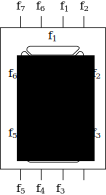
\includegraphics{images/display_7seg}
\end{center}

Cada algarismo hexadecimal é representado por uma combinação de luzes acesas
e apagadas, como pode ser visto abaixo:\\[6pt]

\noindent
\hspace{-4ex}
\includegraphics[scale=0.65]{images/display_0}\hspace{-4ex}
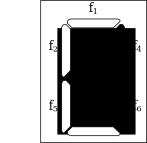
\includegraphics[scale=0.65]{images/display_1}\hspace{-4ex}
\includegraphics[scale=0.65]{images/display_2}\hspace{-4ex}
\includegraphics[scale=0.65]{images/display_3}\hspace{-4ex}
\includegraphics[scale=0.65]{images/display_4}\hspace{-4ex}
\includegraphics[scale=0.65]{images/display_5}\hspace{-4ex}
\includegraphics[scale=0.65]{images/display_6}\hspace{-4ex}
\includegraphics[scale=0.65]{images/display_7}\hspace{-4ex}\\[-6pt]

\noindent
\hspace{-4ex}
\includegraphics[scale=0.65]{images/display_8}\hspace{-4ex}
\includegraphics[scale=0.65]{images/display_9}\hspace{-4ex}
\includegraphics[scale=0.65]{images/display_a}\hspace{-4ex}
\includegraphics[scale=0.65]{images/display_b}\hspace{-4ex}
\includegraphics[scale=0.65]{images/display_c}\hspace{-4ex}
\includegraphics[scale=0.65]{images/display_d}\hspace{-4ex}
\includegraphics[scale=0.65]{images/display_e}\hspace{-4ex}
\includegraphics[scale=0.65]{images/display_f}\hspace{-4ex}

Cada algarismo em hexadecimal pode ser representado por um conjunto de $4$ dígitos $d_3, d_2, d_1, d_0$, da seguinte forma:

\begin{center}
\begin{tabular}{c|c c c c}
algarismo & $d_3$ & $d_2$ & $d_1$ & $d_0$ \\
\hline
0         &   0   &   0   &   0   &   0   \\
1         &   0   &   0   &   0   &   1   \\
2         &   0   &   0   &   1   &   0   \\
\vdots    & \multicolumn{4}{c}{\vdots}    \\
9         &   1   &   0   &   0   &   1   \\
A         &   1   &   0   &   1   &   0   \\
B         &   1   &   0   &   1   &   1   \\
\vdots    & \multicolumn{4}{c}{\vdots}    \\
F         &   1   &   1   &   1   &   1
\end{tabular}
\end{center}

Projete os $7$ circuitos digitais que tenham como entada um algarismo hexadecimal em sua representação binária $d_3 d_2 d_1 d_0$, e que produzem, cada um, uma saída $f_i$ (onde $i = 1\ldots7$), apropriada para um display de $7$ segmentos. Para facilitar, projete e desenhe separadamente cada circuito; antes de desenhar o circuito, simplifique as expressões lógicas para cada $f_i$ usando mapas de Karnaugh (dica: represente diretamente a tabela verdade já como mapa de Karnaugh para economizar tempo e espaço).

\vspace{12pt}

\questao (a) Quantas e quais portas lógicas são usadas em um somador \emph{ripple carry} de $n$ bits que não recebe \emph{carry}
para fazer a soma dos dois algarismos menos significativos?
(b) Quantas e quais portas lógicas são usadas em um somador completo \emph{ripple carry} de $n$ bits (que recebe \emph{carry}
para fazer a soma dos dois algarismos menos significativos)?
Separe as portas lógicas com $2$ entradas das de $3$ entradas.

\vspace{12pt}

\questao Como você juntaria somadores completos de $4$ bits para fazer um somador completo
de $32$ bits?

\vspace{12pt}

\questao Faça o diagrama de um circuito digital para um subtrator de $n$ bits.
Você possui à disposição: um somador completo de $n$ bits; portas NOT.

\vspace{12pt}

\questao Monte um somador binário para números de 5 bits no
Logisim, usando 5 somadores completos de 1 bit. Faça as somas
abaixo usando a representação de complemento de 2 (manualmente e
no Logisim) e interprete os resultados:

\begin{tabular}{p{0.2\textwidth} p{0.2\textwidth} p{0.2\textwidth} p{0.2\textwidth}}
a) $(+3) + (+6)$	&	b) $(-3) + (+6)$	&	c) $(+3) + (-6)$	&	d) $(-3) + (-6)$ \\
e) $(+7) + (+9)$	&	f) $(-7) + (+9)$	&	g) $(+7) + (-9)$	&	h) $(-7) + (-9)$ \\
i) $(-8) + (-9)$
\end{tabular}

\vspace{24pt}

\noindent
Nas questões a seguir, represente os somadores, subtratores, decodificadores e multiplexadores como módulos. Use representação de barramentos quando possível.

\vspace{12pt}

\questao Seja $X = x_{n-1} x_{n-2} \ldots x_1 x_0$ uma palavra
de $n$ bits que representa um número inteiro com sinal no formato de complemento
de $2$. Faça um circuito digital com $n$ entradas e $3$ saídas:
\begin{itemize}
\item $f_{X<0}$, que é $1$ se $X$ representa um número negativo, $0$
caso contrário
\item $f_{X=0}$, que é $1$ se $X$ representa o número zero, $0$
caso contrário
\item $f_{X>0}$, que é $1$ se $X$ representa um número positivo, $0$
caso contrário
\end{itemize}

\vspace{12pt}

\questao Faça um circuito digital com $2n$ entradas e $3$ saídas
$f_{B<A}$, $f_{B>A}$ e $f_{B=A}$ que são $1$, respectivamente, se
$B<A$ ou $B>A$ ou $B=A$, onde $A$, $B$ são palavras de $n$ que representam
números inteiros com sinal no formato de complemento de $2$.

\begin{itemize}
\item Dica: qual é o sinal de $B - A$?

$$
B - A \text{ é } \left\{
\begin{array}{l}
\text{\textbf{negativo} se, e somente se, } B < A \\
= 0 \text{ se, e somente se, } B = A \\
\text{\textbf{positivo} se, e somente se, } B > A
\end{array}
\right.
$$
\end{itemize}

\vspace{12pt}

\questao Faça um circuito para detectar \emph{overflow} em uma
operação de (a) soma e (b) subtração entre duas palavras de $n$ bits
que representam inteiros com sinal no formato complemento de dois.

\vspace{12pt}

\questao Sem usar blocos somadores/subtratores,
faça o diagrama do circuito digital (representado como
``caixa-preta'' na Fig.~\ref{fig:multiplier})
que calcula o produto de dois números inteiros sem sinal com dois
bits cada um. Esse circuito terá 4 entradas e 4 saídas.
\begin{figure}
\begin{center}
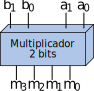
\includegraphics{images/multiplier}
\caption{Multiplicador para dois números de $2$ bits cada um}
\label{fig:multiplier}
\end{center}
\end{figure}

\vspace{12pt}

\questao Faça o diagrama do circuito digital (representado como
``caixa-preta'' na Fig.~\ref{fig:selector}) com $n+1$ entradas,
$x_{n-1}, x_{n-2}, \ldots, x_1, x_0, y$ e $n$ saídas
$z_{n-1}, z_{n-1}, \ldots, z_1, z_0$ tal que:
$$
\text{para todo } i \text{ entre } 0 \text{ e } n-1 \text{, }
z_i = \left\{
 \begin{array}{l}
   0 \text{ se } y = 0 \\
   x_i \text{ se } y = 1
 \end{array} \right.
$$
(resolva primeiro para $1$, $2$, $3$, \ldots)
\begin{figure}
\begin{center}
\includegraphics{images/selector}
\caption{Seletor}
\label{fig:selector}
\end{center}
\end{figure}

\vspace{12pt}

\questao (a) Faça um multiplicador para dois números sem sinal de
dois bits cada, agora usando blocos somadores. (b) Idem, mas agora
para números de $n$ bits sem sinal (pode ajudar se você pensar nos
casos particulares primeiro: $n = 3$, $n = 4$, \ldots)

\vspace{12pt}

\questao Faça os diagramas dos circuitos para os codificadores
2 para 1, 4 para 2 e 8 para 3 com entradas: (a) ativas em nível alto;
(b) ativas em nível baixo.

\vspace{12pt}

\questao (a) Construa um MUX $16\times1$ com multiplexadores $4\times1$.
(b) Construa um MUX $16\times1$ com multiplexadores $2\times1$.

\vspace{12pt}

\questao Faça os circuitos para os demultiplexadores: (a) $1 \times 2$;
(b) $1 \times 4$; (c) $1 \times 8$;\\ (d) $1 \times 16$. Dica: use
decodificadores.

\vspace{12pt}

\questao (a) Construa um circuito digital que transforme uma palavra de $n$ bits
contendo um inteiro com sinal no formato sinal-magnitude para o formato
complemento de dois. (b) Construa um circuito que faça a conversão contrária.
Para facilitar, ignore em (a) e (b) os casos em que
a conversão possa resultar em \emph{overflow}. Os blocos lógicos disponíveis
para utilização são: somador de $n$ bits, bitwise AND/OR/NOT de $n$ bits,
MUX $2\times1$ de $n$ bits e portas lógicas AND/OR/NOT/NAND/NOR/XOR/XNOR.

\vspace{12pt}

\questao (a) Construa um circuito digital que converta uma palavra de $4$ bits
contendo um inteiro com sinal no formato complemento de dois para $8$ bits,
no mesmo formato. (b) Construa um circuito digital que converta uma palavra de
$8$ bits contendo um inteiro com sinal no formato complemento de dois para $4$ bits,
no mesmo formato. (c) Generalize os circuitos em (a) e (b) para fazer as conversões
de $n$ para $2n$ bits e vice-versa.
Para facilitar, ignore em (a), (b) e (c) os casos em que
a conversão possa resultar em \emph{overflow}. Os blocos lógicos disponíveis
para utilização são: somador de $n$ bits, bitwise AND/OR/NOT de $n$ bits,
MUX $2\times1$ de $n$ bits e portas lógicas AND/OR/NOT/NAND/NOR/XOR/XNOR.

\vspace{12pt}

\questao Construa um circuito digital com $7$ entradas $a_5 \ldots a_0$, $op$ e $6$ saídas $s_5 \ldots s_0$ tais que:

\begin{itemize}
\item $a_5 \ldots a_0$ representa um número inteiro sem sinal $A$ em $6$ bits;
\item $op$ indica a operação a ser executada: se $op = 0$, obtém o resultado da multiplicação $2A$ (apenas os $6$ bits menos significativos); se $op = 1$, obtém o quociente inteiro da divisão $A/2$
\item $s_5 \ldots s_0$ é o resultado da operação
\end{itemize}

Os blocos lógicos disponíveis
para utilização são: somador de $n$ bits, bitwise AND/OR/NOT de $n$ bits,
MUX $2\times1$ de $n$ bits e portas lógicas AND/OR/NOT/NAND/NOR/XOR/XNOR.

(dica: o que acontece quando multiplicamos um número em binário por $2$? e quando dividimos por $2$?)

\vspace{12pt}

\questao Construa um circuito com:
\begin{itemize}
\item $8$ entradas de dados $b_3, b_2, b_1, b_0$, $a_3, a_2, a_1, a_0$
\item $2$ entradas de seleção $Op_1, Op_0$
\item $4$ saídas $s_3, s_2, s_1, s_0$
\end{itemize}
tal que $$
(s_3 s_2 s_1 s_0)_2 = \left\{
\begin{array}{ll}
(b_3 b_2 b_1 b_0)_2 + (a_3 a_2 a_1 a_0)_2 & \text{se } (Op_1 Op_0)_2 = 0 \\
(b_3 b_2 b_1 b_0)_2 - (a_3 a_2 a_1 a_0)_2 & \text{se } (Op_1 Op_0)_2 = 1 \\
(a_3 a_2 a_1 a_0)_2 + 1 & \text{se } (Op_1 Op_0)_2 = 2 \\
(a_3 a_2 a_1 a_0)_2 - 1 & \text{se } (Op_1 Op_0)_2 = 3 \\
\end{array}
\right.
$$
Todas as operações são com números sem sinal. Desconsidere os casos em que há overflow.


\vspace{12pt}

\questao Construa um circuito digital com $2n + 1$ entradas $a_{n-1} \ldots a_0$, $b_{n-1} \ldots b_{0}$, $op$ e $n+1$ saídas $s_{n-2} \ldots s_0$, $err$ tais que:

\begin{itemize}
\item $A = a_{n-1} a_{n-2} \ldots a_0$ e $B = b_{n-1} b_{n-2} \ldots b_{0}$ são dois números com $n$ bits em binário em complemento a $2$ (os bits mais significativos, respectivamente $a_{n-1}$ e $b_{n-1}$, indicam o sinal);
\item $op$ indica a operação a ser executada: se $op = 0$, então é feita a soma $A+B$; se $op = 1$ então é feita a subtração $A - B$;
\item $s_{n-1} \ldots s_0$ é o resultado da operação, com $n$ bits, em complemento a $2$ ($s_{n-1}$ indica o sinal);
\item $err$ é um indicador de \emph{overflow} ou \emph{underflow}. Ele será $1$ se a soma $A+B$ excede $n-1$ bits ou se a subtração $A - B$ resulta em um número menor do que $-2^{n-1}$ (condição de \emph{underflow}, o resultado não pode ser representado em $n$ bits usando complemento a $2$).
\end{itemize}

Os blocos lógicos disponíveis
para utilização são: somador de $n$ bits, bitwise AND/OR/NOT de $n$ bits,
MUX $2\times1$ de $n$ bits e portas lógicas AND/OR/NOT/NAND/NOR/XOR/XNOR.

\end{document}

